% 1979 年全国卷文科第 7 题：已知圆的内接矩形 CEDF，过 D 的切线（直线 AB）与 CE 的延长线交于 A、与 CF 的延长线交于 B；连 CD（虚线，直径）；源卷图无圆点、无圆心标记，故不标（按源卷布局）
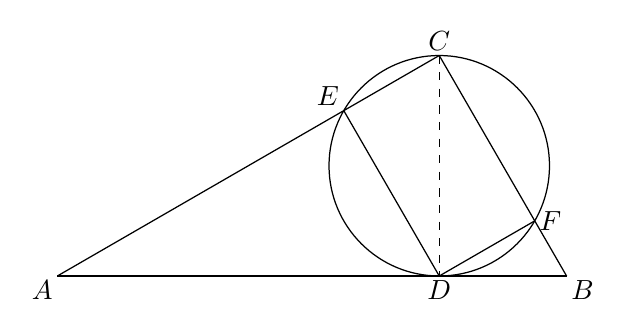
\begin{tikzpicture}[scale=1.4, line width=0.45pt,
  every node/.style={inner sep=1.5pt}]
  \coordinate (A) at (-3.464,-1);
  \coordinate (B) at (1.155,-1);
  \coordinate (C) at (0,1);
  \coordinate (D) at (0,-1);
  \coordinate (E) at (-0.866,0.5);
  \coordinate (F) at (0.866,-0.5);
  \draw (0,0) circle (1);
  \draw (A) -- (B);
  \draw (A) -- (C);
  \draw (B) -- (C);
  \draw (E) -- (D);
  \draw (D) -- (F);
  \draw[dashed] (C) -- (D);
  \node[anchor=north east] at (A) {$A$};
  \node[anchor=north west] at (B) {$B$};
  \node[anchor=south] at (C) {$C$};
  \node[anchor=north] at (D) {$D$};
  \node[anchor=south east] at (E) {$E$};
  \node[anchor=west] at (F) {$F$};
\end{tikzpicture}
